\documentclass{article}
\usepackage{graphicx} % Required for inserting images

\usepackage{darkmode}
\enabledarkmode

\usepackage{amsmath}
\usepackage{tikz}
\usepackage{framed}
\usepackage{pgfplots}
\usepackage{pgfplotstable}
\usepackage{mdframed}
\usepackage{textcomp}
\usepackage{ulem}
\usepackage{cancel}

\usetikzlibrary{3d, positioning}


\begin{document}
    \section{Center of Mass}
        \subsection{Discrete}
        \begin{equation}
            \large
            R_{cm} = \frac{1}{M_{total}} \sum_{n=1}^{N} m_n r_n
        \end{equation}
        \hfil

        Find a point in the center of a group of points. 

        \hrulefill
        \subsection{\centering \huge Examples}
        \hrulefill

        \subsubsection{\centering Example one}
        \hrulefill

        \begin{center}
            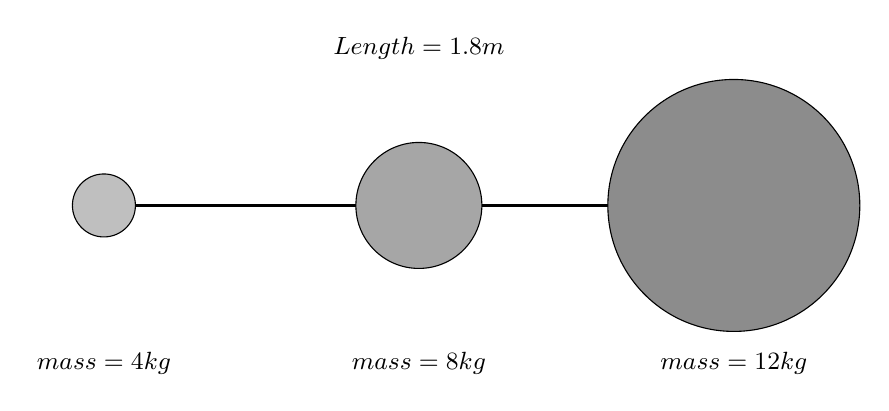
\begin{tikzpicture}[scale=.4]
                % Define the positions
                \draw[thick] (-10,0) -- (10,0); % Draw a horizontal reference line
                
                % Draw circles with specified radii
                \draw[fill=gray!50] (-10, 0) circle (1);  % First ball with radius 4
                \draw[fill=gray!70] (0, 0) circle (2);   % Second ball with radius 8
                \draw[fill=gray!90] (10, 0) circle (4);  % Third ball with radius 12
            
                % Labels for clarity
                \node at (-10, -5) {\small $mass=4kg$};
                \node at (0, -5) {\small $mass=8kg$};
                \node at (10, -5) {\small $mass=12kg$};
                \node at (0, 5) {\small $Length = 1.8m$};

            \end{tikzpicture}
        \end{center}
        \[\boxed{x_{cm} = \frac{x_1m_1 + x_2m_2+ x_3m_3 }{m_1+ m_2 + m_3}}\]

        \[\boxed{x_{cm} = \frac{(0)(4) + (.9)(8) + (1.8)(12) }{4 + 8 + 12}}\]
        
        \subsubsection{Example Two}
        \hrulefill

            \begin{center}
                \begin{tabular}{|| c c c c c ||}
                    \hline
                    m & x & y & $v_x$ & $v_y$  \\ 
                    \hline
                    1 & 7.8 & -2.8 & 3.2 & -4.2 \\  
                    2 & 7.8 & -3.7  & -5.2 &  5.2 \\
                    3 & 7.8 & -5.7  & -6.2 &  2.2 \\ 
                    4 & 7.8 & 2.7  & 4.2 & -3.2 \\
                    \hline
                \end{tabular}
            \end{center}
        
           \[\boxed{x_{cm} = \frac{x_1m_1 + x_2m_2+ x_3m_3 + x_4m_4}{m_1+ m_2 + m_3 +m_4}}\]


        \subsection{Example Three}
        \hrulefill \\ [20pt]


            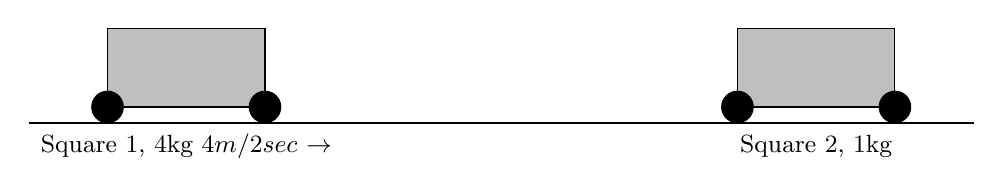
\begin{tikzpicture}
                % Draw a horizontal reference line
                \draw[thick] (-6,-.2) -- (6,-.2);
                
                % Draw two squares, 10 units apart
                
                \draw[fill=gray!50] (-5,0) rectangle (-3,1); % First square
                \draw[fill=gray!50] (3,0) rectangle (5,1);   % Second square
                
                \draw[fill=black] (-5,0) circle (.2);
                \draw[fill=black] (-3,0) circle (.2);
                \draw[fill=black] (3,0) circle (.2);
                \draw[fill=black] (5,0) circle (.2);
                % Labels
                \node at (-4, -.5) {\small 
                
                Square 1, 4kg \\ [10pt]
                $4m/2sec$ $\rightarrow$\\};
                \node at (4, -.5) {\small Square 2, 1kg};
            \end{tikzpicture}

            \begingroup 
                \large
                \begin{center}
                    $X_{cm} = \frac{x_1m_1+x_2m_2}{m_1 + m_2 }$\\[15pt]
                    $V_{cm} = \frac{v_1m_1+v_2m_2}{m_1 + m_2 }$\\[15pt]

                    $X_{cm} = \frac{(4)(3) + (1)(0)}{(4 + 1)}$\\[15pt]
                    
                    $V_{LAB} = 2.4 m/s$ \\
                    $V_{CM} = -2.4 m/s$ \\[10pt]

                    $V_{b_1CM} = V_{b_1LAB} + V_{LAB_1CM}$\\
                    $ 3m/s - 2.4m/s$\\
                    $V_{b_1}cm = .6m/s$\\[10pt]

                    $V_{R_1CM} = V_{R_1LAB} + V_{LAB_1CM}$\\
                    $ 0m/s - 2.4m/s$\\
                    $V_{R_1}cm = -2.4m/s$\\

                \end{center}
                
                
                
            \endgroup
     
        \pagebreak



        \subsection{Continuous}
        \[R_{cm} = \frac{1}{M_{total}} \int \vec{r}dm\]

        \subsection{COM of multiple objects}


    \pagebreak
    \section{\huge Momentum}
    \hrulefill
    \begin{equation}
        \huge
        \boxed{\vec{P} = m\vec{v}}
    \end{equation}

    \begin{center}
        \textit{Different version of Newtons law.}
    \end{center}
    
    \begin{center}
        \large
        \fbox{$\vec{P_{total}} = M_{total}V_{cm}$} \\ [15pt]

        $P_i = P_f$\\[15pt]

        $ {m_1v_1}_i +{m_2v_2}_i ={ m_1v_1}_f + {m_2v_2}_f $\\[15pt]

        \fbox{Special Case Eqs}\\ [15pt]
        $v_{1f} = \frac{v_{1f}(m_1-m_2)} {(m_1 + m_2)}$ \\ [15pt]

        $v_{2f} = \frac{v_{1f}(2m)} {(m_1 + m_2)}$ \\ [15pt]
    \end{center}

    
    \hrulefill
    \subsection{Elastic Collisions}
        \begin{list}{-}{}
            \item Conservation of linear Momentum
            \item conservation of mechanical energy
            \item kinetic energy of the system is conserved, 
            \item kinetic energy of the individual bodies can change
            \item ex. Billiard ball collisions
        \end{list}
    \subsection{Inelastic Collisions}
        \begin{list}{-}{}
            \item Mechanical energy not conserved 
            \item conservation of linear Momentum
            \item loss of energy: sound, heat, Elastic, Etc 
            \item bodies stick together 
            \item paintball
        \end{list}

    In a closed system, no momentum will be  lost. 

    \begin{list}{-}{}
        \item Friction is typically not considered 
        \item typically the system will have a net force
    \end{list}

    \subsection{Center of Mass Frame}
    In center of mass frame, Velocity is equal to zero. \\ [20pt]

    \begingroup 
    \centering
    \large
    $V_{cm} = \frac{v_1m_1+v_2m_2}{m_1 + m_2 }$\\[15pt]
    \endgroup

    COM Ref frame will stay in the same spot before and after collision. 
    Magnitude of initial v1 will be equal to v2f. \\

    \begingroup 
    \centering
    \large
    $|v_{1_i}| =|v_{1_f}|$ \\ [10pt]
    $|v_{2_i}| =|v_{2_f}|$ \\ [20pt]
    \endgroup


    \begingroup
    \centering
        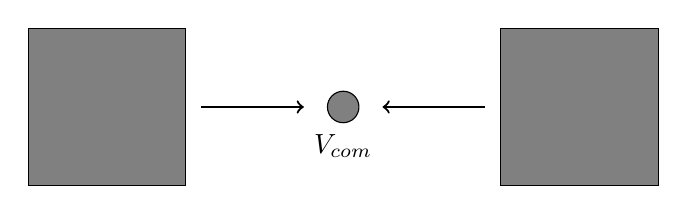
\begin{tikzpicture}
            \draw[fill = gray] (-4,-1) rectangle (-2,1);
            \draw[->, thick] (-1.8,0) -- (-.5, 0);
            \draw[fill = gray] (0,0) circle (.2);
            \node at (0,-.5) {$V_{com}$};
            \draw[fill = gray] (4,-1) rectangle (2,1);
            \draw[->, thick] (1.8,0) -- (.5, 0);
        \end{tikzpicture} \\ [15pt]

        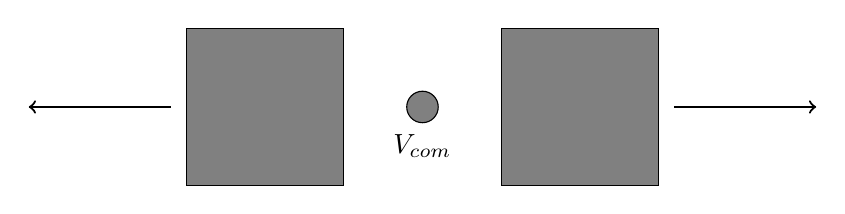
\begin{tikzpicture}
            \draw[fill = gray] (-3,-1) rectangle (-1,1);
            \draw[->, thick] (-3.2,0) -- (-5, 0);
            \draw[fill = gray] (0,0) circle (.2);
            \node at (0,-.5) {$V_{com}$};
            \draw[fill = gray] (3,-1) rectangle (1,1);
            \draw[->, thick] (3.2,0) -- (5, 0);


        \end{tikzpicture} \\ [15pt]
    \endgroup

    Thus, you can just convert to COM ref frame and then just  




\pagebreak


 
\subsection{\huge \centering Examples}
\hrulefill
\centering
\subsubsection{\fbox{Example 1}}
\hrulefill

A 3kg cart is rolling along when a at 5m per sec a 2kg drops on tp of and sticks

what is the final velocity 

$p_i = m_1v_1 +m_2v_2$

$=(3)(5)$

$P_f = (m_1+ m_2) V_f$

$\rightarrow$

$V_f = 3m/s$ \\[30pt]

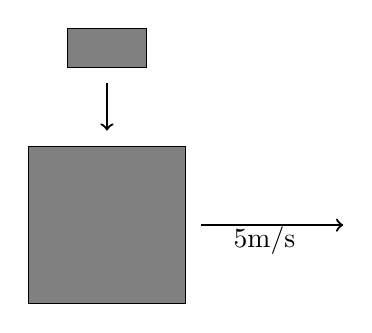
\begin{tikzpicture}
    \draw[fill = gray] (-1,-1) rectangle (1,1);
    \draw[->, thick] (0, 1.8) -- (0, 1.2);
    \draw[fill = gray] (-.5,2) rectangle (.5,2.5);
    \draw[->, thick] (1.2, 0) -- (3, 0);
    \node at (2, -.2) {5m/s};
\end{tikzpicture}

\hrulefill
\subsubsection{\fbox{Example 2}}
\hrulefill \\[15pt]

Train cars are coupled together by being bumped into each other. Supposed two loaded train cars are moving towards each there, first having a mass of $1.5 x 105kg$ and a velocity of $.3m/s \hat{i}$ and the second having a mass of $1.1x105kg$ and a velocity of $-.12m/s \hat{j}$\\[20pt]

\textbf{\large Before}\\
$P_i = m_1v_1 +m_2v_2$\\[15pt]

\textbf{\large Ater}\\
$P_f = (m_1+ m_2) V_f$\\[15pt]

$P_i = P_f$\\[15pt]

$P_i = m_1v_1 +m_2v_2$ = $P_f = (m_1+ m_2) V_f$\\[15pt]

$V_{cm} = \frac{v_1m_1+v_2m_2}{m_1 + m_2 }$\\[15pt]


\hrulefill
\subsubsection{\fbox{Example 3, Ballistic Pendulum $\star$}}
\hrulefill \\[15pt]

A projectile of mass $m$ moving horizontally with speed $v$ strikes a stationary mass $M$ suspended by strings of length $L$. Subsequently, $m+M$ rise to a height of $H$

\textit{perfectly inelastic collision}\\[20pt]

$P_i = P_f $\\[15pt]

$Mv_i = (m+M)v_f$\\[15pt]

$V_f = \frac{mv_i}{m+M}$\\[15pt]

$(m+M)gH = \frac{1}{2}(m+M)v^2$\\[15pt]

$H= \frac{v^2}{2g} - \frac{\frac{(mV)^2}{(m+M)^2}}{2g} = \frac{(m^2v^2)}{2((m+M)^2)g}$\\[15pt]

\hrulefill\\[15pt]

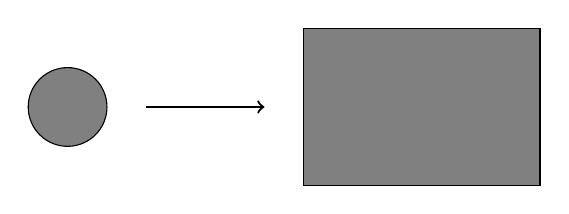
\begin{tikzpicture}

    \draw[fill = gray, anchor = center ] (3,1) rectangle (0,-1);
    \draw[fill = gray, anchor = center] (-3,0) circle (.5);
    \draw[->, thick] (-2, 0) -- (-.5, 0);
\end{tikzpicture}

\pagebreak
\hrulefill
\subsubsection{\fbox{Example 4}}
\hrulefill \\[15pt]

The figure below (bullet hitting block) shows a bullet of mass 200g traveling towards the east with a speed of $400m/s$, which stirks a block of  mass 1.5kg that is intentionally at rest on a frictionless table \\[15pt]

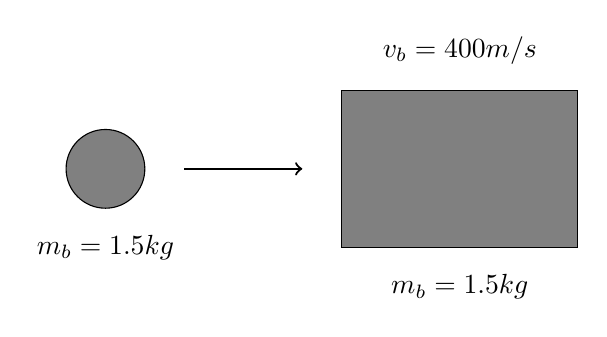
\begin{tikzpicture}
    \draw[fill = gray, anchor = center ] (3,1) rectangle (0,-1);
    \node at (1.5,1.5) {$v_b = 400m/s$};
    \node at (1.5,-1.5) {$m_b = 1.5kg$};
    \draw[fill = gray, anchor = center] (-3,0) circle (.5);
    \node at (-3,-1) {$m_b = 1.5kg$};
    \draw[->, thick] (-2, 0) -- (-.5, 0);
\end{tikzpicture}

\hrulefill
\subsubsection{\fbox{Example 5}}
\hrulefill \\[15pt]

A glider of mass .02 kg slides on a frictionless track with initial velocity of 1.5 m/s. It hits a glider of mass .8kg moving to the left at v2i = .2m/s. A spring attached to the first glider compresses and relaxes during the collision, but this is no friction (energy is conserved). What are the final velocities. \\ [15pt]

\fbox{\textit{Special Case Eqs}} \\ [10pt]

$v_{1f} = \frac{v_{1f}(m_1-m_2)} {(m_1 + m_2)}$ \\ [15pt]

$v_{2f} = \frac{v_{1f}(2m)} {(m_1 + m_2)}$ \\ [15pt]

$v_{2f} = \frac{(1.5)(.4)} {(1)} = .6$\\ [15pt]

$v_{1f} = \frac{(1.5)(-.6)} {(1)} = -.9kg$\\ [15pt]

\pagebreak
\subsection{\huge Moment of inertia}
    \hrulefill \\
    $I = I_c + MD^2$ \\
    $x \rightarrow \theta$ \\
    $dx/dt = v \rightarrow d\theta/dt = \omega$ \\
    $m = I$ \\
    \hrulefill
        

    \subsubsection{\large \centering Examples}
    \hrulefill
    \centering
    \subsubsection{\fbox{Example 1}}
        What is the moment of inertia of two solid spheres with radius r = 10cm and mass 10kg. Attached to a rod of mass 2kg and length of d = 25cm
        \\ [15pt]
        $I_{system} = I_{sphere} + I_{sphere_2} + I_{rod}$ v \\[10pt]
        $= 2(i_{sphere_cm} + MD^2) + I_{rod_{cm}}$   \\[10pt]
        $ = 2(\frac{2}{5}MR^2 + M(R+\frac{d}{2})^2 + \frac{1}{12}md^2)$ \\ [10pt]
        $=2(\frac{2}{5})(10)(.1)^(.1) + (10)(.225)^2 + \frac{1}{12}(2)(.25)^2$ \\ [10pt]
        $I_{system} = 1.103kgm^2$ \\ [20pt]

        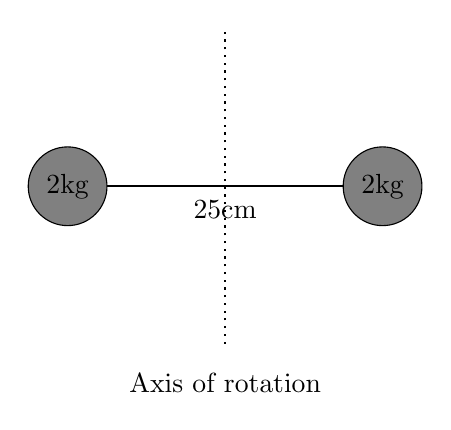
\begin{tikzpicture}
            \draw[-, thick] (-2, 0) -- (2,0);
            \draw[dotted, thick] (0, -2) -- (0,2);
            \draw[fill = gray, anchor = center] (-2,0) circle (.5);
            \draw[fill = gray, anchor = center] (2,0) circle (.5);
            \node at (0, -2.5) {Axis of rotation};
            \node at (0, -.3) {25cm};
            \node at (-2, 0) {2kg};
            \node at (2, 0) {2kg};
        \end{tikzpicture}

    \hrulefill
    \subsubsection{\huge Torque}
        $|\tau| = |r| |F| \sin{\theta}$ \\
        $\vec{\tau} = \vec{r}X\vec{F}$ \\ 
        $W = \vec{\tau}\Delta\vec{\theta}$ \\

        $KE_{total} = KE_{tras} + KE_{rot}$ \\
         $=1/2mv^2_{com} +1/2I_{com}W^2$\\

        \textbf{Kinematic equations }
        \begin{align}
            \omega &= \omega_0 + \alpha t \\
            \theta &= \omega_0 t + \frac{1}{2} \alpha t^2 \\
            \omega^2 &= \omega_0^2 + 2\alpha \theta \\
            \theta &= \frac{1}{2} (\omega + \omega_0) t \\
            \theta &= \omega t - \frac{1}{2} \alpha t^2
            \end{align}
            
    \hrulefill

    \subsection{\large \centering Examples}
    \hrulefill
    \centering
    \subsubsection{\fbox{Example 1}}   
        A 50n force is placed on one end of a 25cm long wrench as shown. what is the torque applied by this force if it rotates about the other end? \\ [20pt]

        \begingroup
        \centering

        $\tau = (.25m)(50n)(\sin120)$ \\[10pt]

        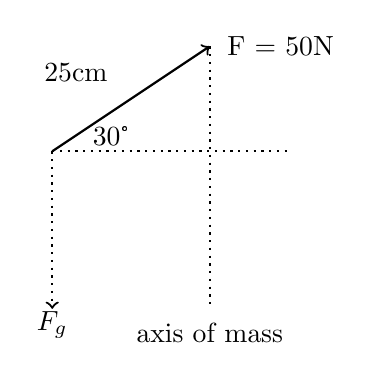
\begin{tikzpicture}
            \draw[->, thick] (0, 0) -- (2,1.333);
            \node at (.75,.2) {30\textdegree};
            \node at (.3,1) {25cm};
            \draw[dotted, thick] (0, 0) -- (3,0);
            \draw[dotted, thick] (2, 1.333) -- (2,0-2);
            \node at (2,0-2.3) {axis of mass};
            \node at (2.9, 1.333) {F = 50N};
            \draw[->, dotted, thick] (0, 0) -- (0,-2);
            \node at (0,-2.2) {$F_g$};
        \end{tikzpicture}
        \endgroup

        \hrulefill

        \subsubsection{\fbox{Example 2}}
            A long length of string is wrapped around 5kg drum with a radius of 30cm. The drum is free to spin around a frictionless axle. The other end of the string is attached to a 10kg mass. If the mass is allowed to drop, what is the acceleration?

            $a_t = R \alpha \rightarrow \alpha = \frac{a}{r}$\\ [10pt]
            $I_{soliddisk} = \frac{1}{2} M_1R^2$ \\ [10pt]
            $\sum F = M_2a$  \\ [10pt]
            $M_2g - T = M_2a$\\[10pt]
            $T = m_2g = m_2a$ \\[10pt]
            \hrulefill \\[10pt]
            $\sum\tau = I \alpha$\\[10pt]
            $\cancel{\tau_{fg}} + \cancel{\tau_{Fs}} + \tau_T = \frac{1}{2} M_1R^2\frac{a}{R}$ \\ [10pt]
            $T\cancel{R} = \frac{1}{2} M_1\cancel{R}^2\frac{a}{\cancel{R}}$\\[10pt]
            $T = \frac{1}{2} m_1a$ \\[20pt]
            \hrulefill \\[10pt]
            $\frac{1}{2} m_1a = m_2g = m_2a $ \\ [15pt]

            $a = \frac{M_2g}{\frac{1}{2}M_1 +M_2}$ \\[20pt]




            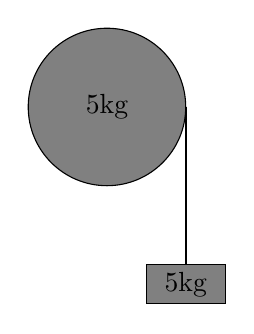
\begin{tikzpicture}
                \draw[fill = gray, anchor = center] (0,0) circle (1);
                \node at (0,0) {5kg};
                \draw[-, thick] (1,0) -- (1,-2);
                \draw[fill = gray, anchor = center] (.5,-2) rectangle (1.5, -2.5);
                \node at (1,-2.25) {5kg};

            \end{tikzpicture}\\ [15pt]
        \hrulefill
        \subsubsection{\fbox{Example 3}}
        \hrulefill
        A long length of string is wrapped around a 5kg drum with a radius of 30cm. The drum is free to spin around a frictionless axle. After the string has been pulled with a 10n force for a distance of 5m. What is the angular velocity of the drum.

        $W_{net} = \Delta~KE$ \\ [10pt]

        $F \times d = RKEf - \cancel{Rkei} $\\ [10pt]
        $F \times d= \frac{1}{2} IW_f^2$ \\ [10pt]

        $I = \frac{1}{2}MR^2 = \frac{1}{2} (5kg)(.3m)^2$ \\ [10pt]
        $I = .225Kgm^2$ \\ [10pt]

        $(10N)(5m) = \frac{1}{2}(.225kgm^2)W_f^2$ \\ [10pt]
        $W_f = 21.1 \frac{Rad}{S}$

        \hrulefill
        \subsubsection{\fbox{Example 4}}
        \hrulefill \\
            A length of string is wrapped around a 5kg drum with a radius of 30cm. The drum is free to spin around a frictionless axle. The other end of the string is attached to a 10kg mass. What is the angular velocity of the pully after the mass has dropped 2m? \\
            [15pt]
        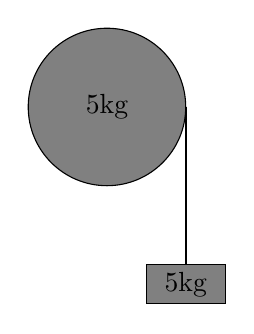
\begin{tikzpicture}
            \draw[fill = gray, anchor = center] (0,0) circle (1);
            \node at (0,0) {5kg};
            \draw[-, thick] (1,0) -- (1,-2);
            \draw[fill = gray, anchor = center] (.5,-2) rectangle (1.5, -2.5);
            \node at (1,-2.25) {5kg};

        \end{tikzpicture}\\ [15pt]

        $W_f^2 = \cancel{W_0^2} +2\alpha~\Delta~\theta$ \\[10pt]
        $W_f = \sqrt{2(26.1\frac{rad}{s^2}(6.66rad))}$ \\[15pt]
        $W_f = 18.6 \frac{rad}{s}$ \\

        $rev = 2\pi~R$ \\ [15pt]
        $= 2\pi~(.3)$ \\ [10pt]
        $=.6\pi\omega$ \\[10pt]
        $=2.0\omega$ \\[10pt]
            



\end{document}